\thispagestyle{fancy}

\vspace*{\fill}

\subsection{Tela comandos de máquina}

Para acessar esta tela da inicial basta clicar em comandos no menu inferior. Ao iniciar a máquina com exceção da tela de ajuda, alarmes e velocidade; esta é a única tela é possível acessar com a máquina desabilitada. Ao habilitar a máquina o menu de ajustes, pedido, configuração, a tela de comandos das outras unidades e próxima página de comandos de máquina ficam disponíveis.

O menu superior esquerdo leva a tela de comandos de cada uma das unidades, o botão "\textgreater" no menu superior esquerdo leva a tela de comandos da alimentação, o botão "\textgreater" no canto direito leva a segunda tela de comandos de máquina e o "ajustes" como não existe uma tela de ajuste de máquina leva a tela de ajustes da alimentação.

\vspace*{10pt}

\begin{figure}[h]
  \centering
  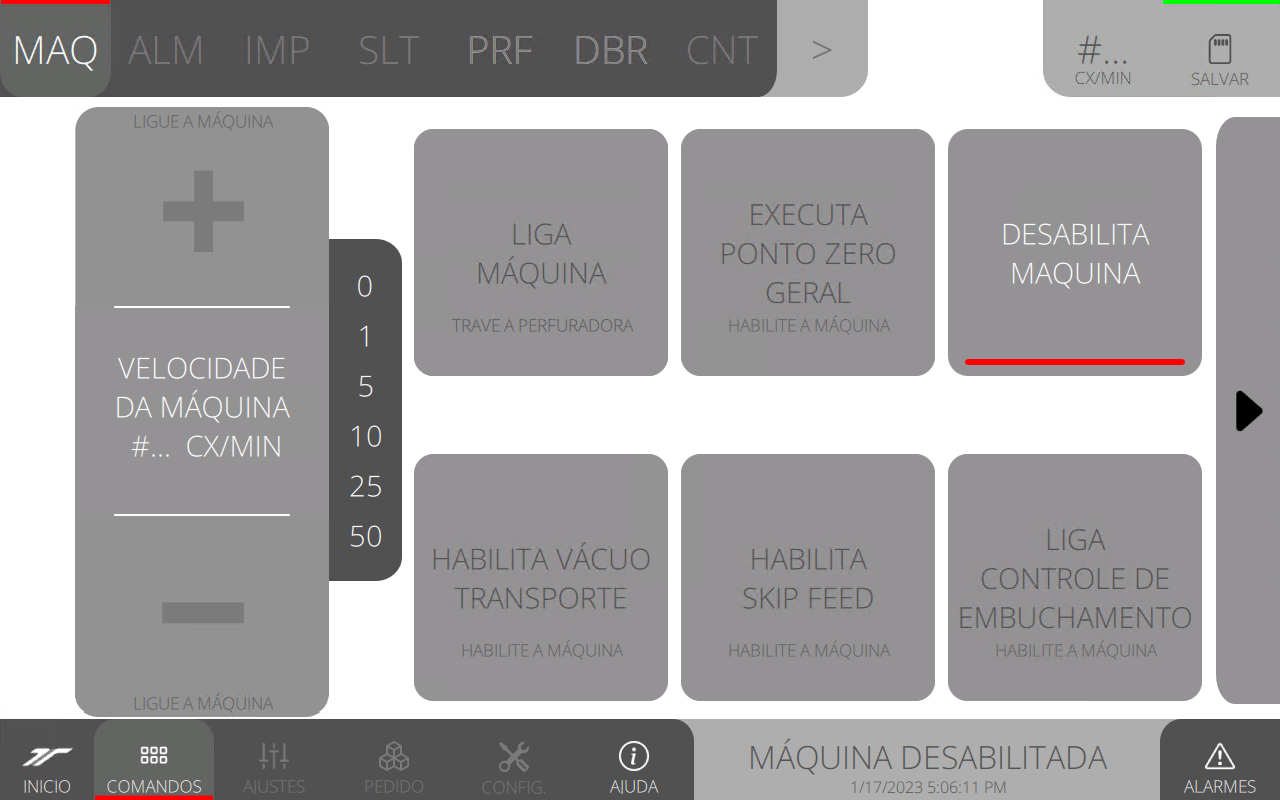
\includegraphics[width=480px,height=300px]{src/imagesFlexo/02-machine/e-Tela-Principal.png}
\end{figure}

\vspace*{\fill}

\newpage
\thispagestyle{fancy}

\vspace*{\fill}

\subsubsection{\small{Acesso rápido à velocidade da máquina}}

\begin{figure}[h]
  \centering
  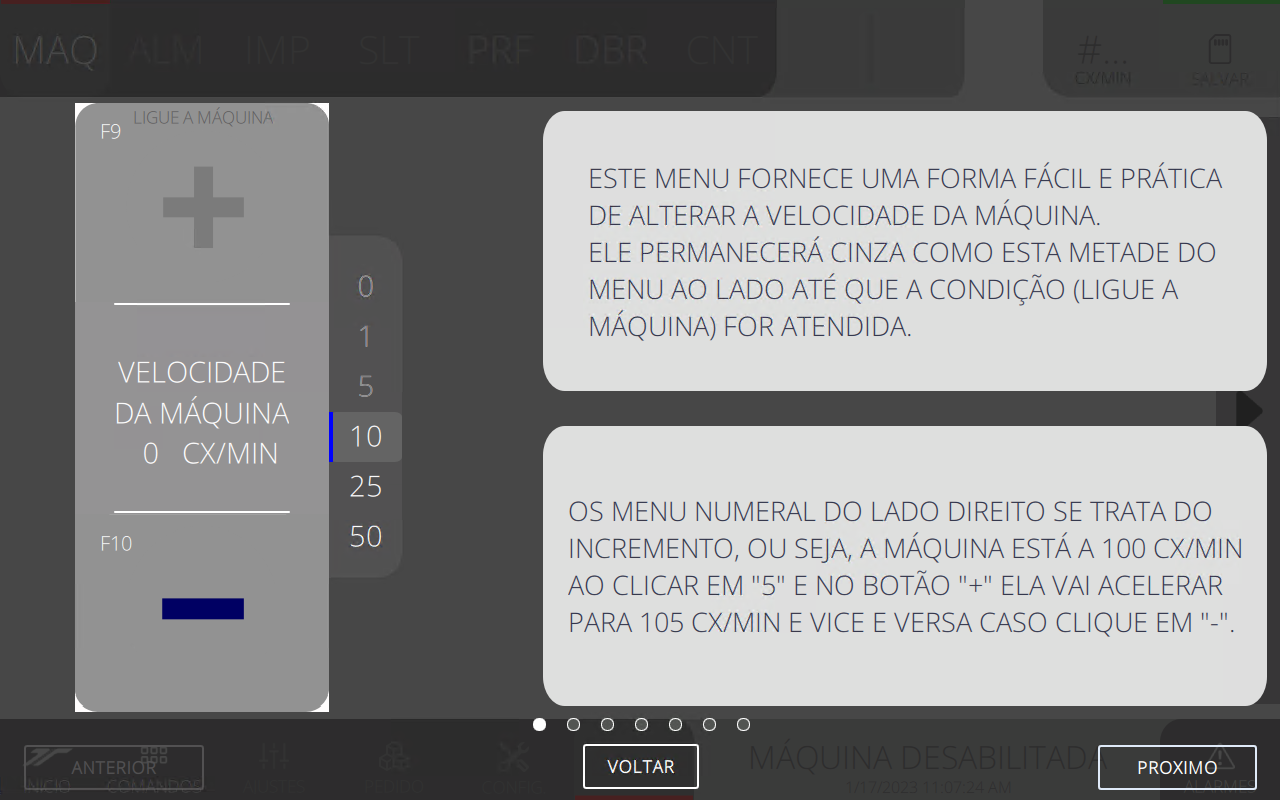
\includegraphics[width=576px,height=360px]{src/imagesFlexo/02-machine/e-1.png}
\end{figure}

\vspace*{\fill}

\newpage
\thispagestyle{fancy}

\vspace*{\fill}

\subsubsection{\small{Liga máquina}}

\begin{figure}[h]
  \centering
  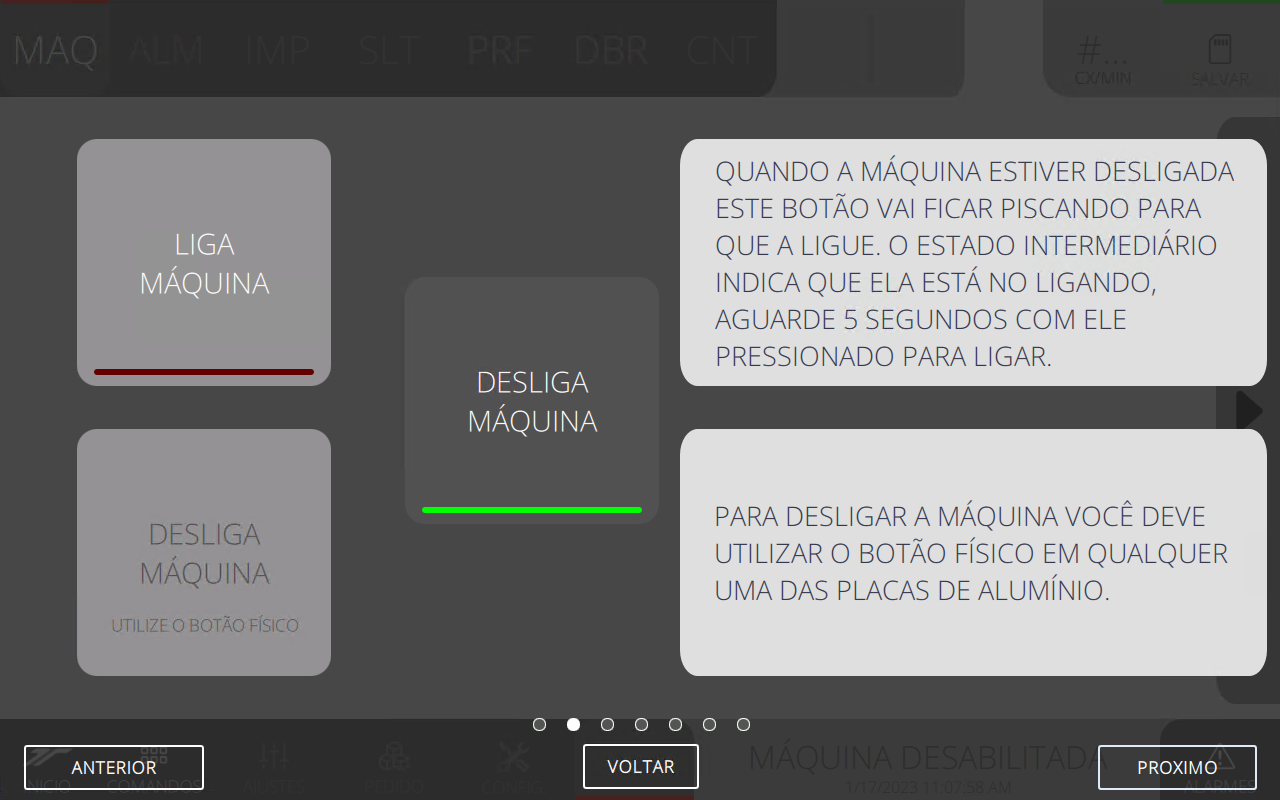
\includegraphics[width=576px,height=360px]{src/imagesFlexo/02-machine/e-2.png}
\end{figure}

\vspace*{\fill}

\newpage
\thispagestyle{fancy}

\vspace*{\fill}

\subsubsection{\small{Ponto zero geral}}

\begin{figure}[h]
  \centering
  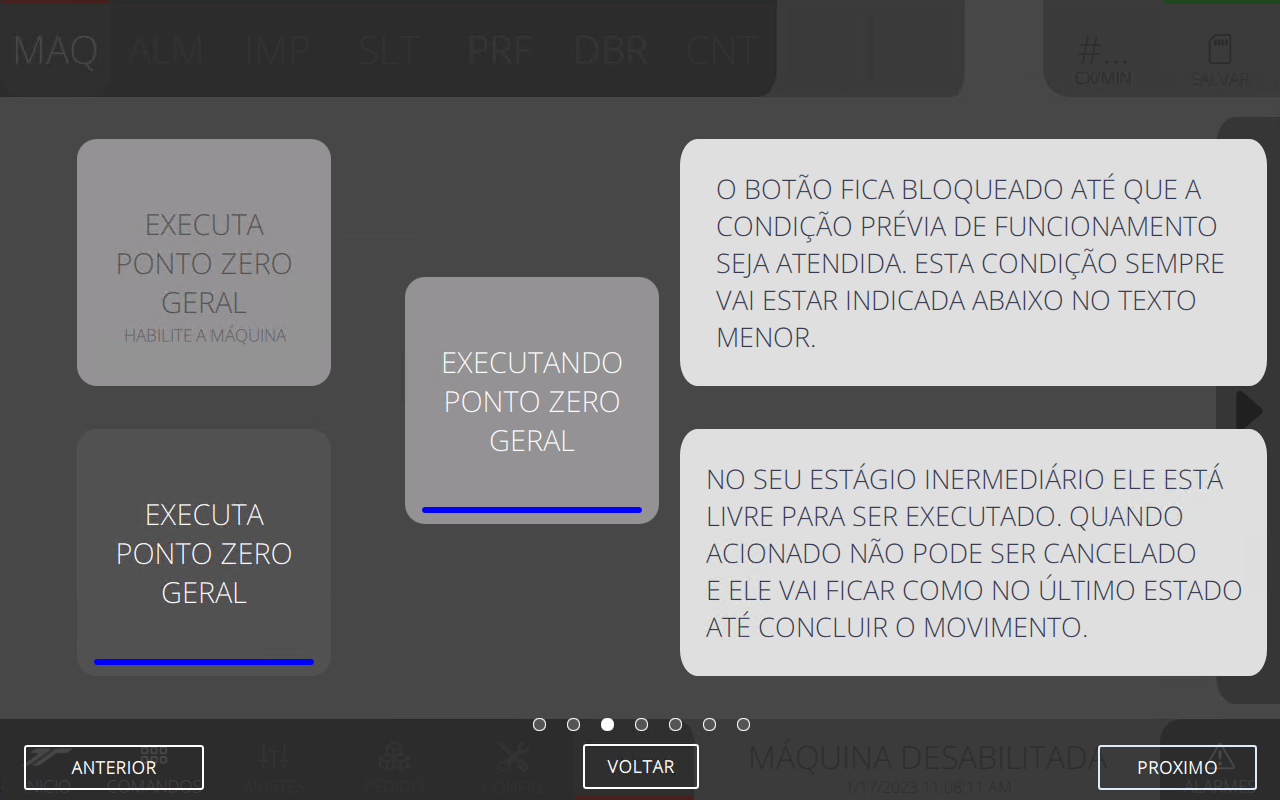
\includegraphics[width=576px,height=360px]{src/imagesFlexo/02-machine/e-3.png}
\end{figure}

\vspace*{\fill}

\newpage
\thispagestyle{fancy}

\vspace*{\fill}

\subsubsection{\small{Habilita máquina}}

\begin{figure}[h]
  \centering
  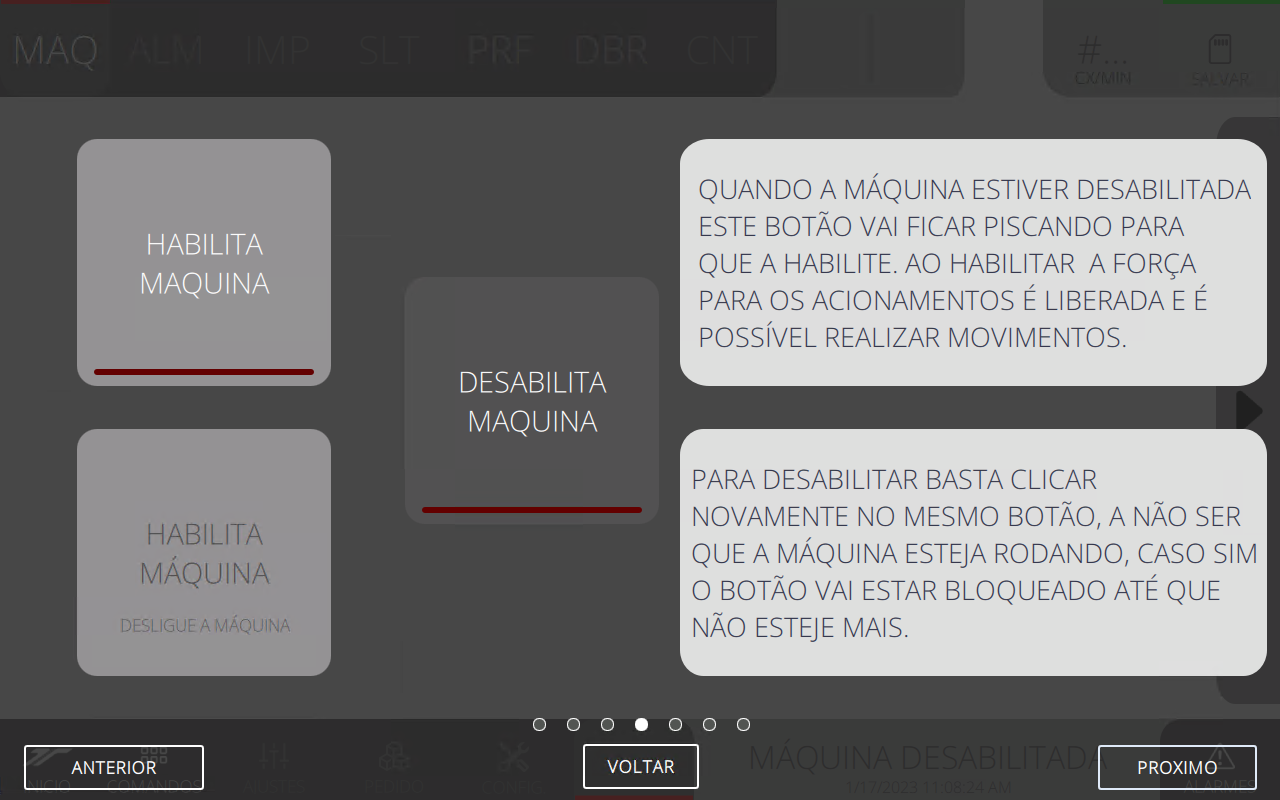
\includegraphics[width=576px,height=360px]{src/imagesFlexo/02-machine/e-4.png}
\end{figure}

\vspace*{\fill}

\newpage
\thispagestyle{fancy}

\vspace*{\fill}

\subsubsection{\small{Habilita vácuo transporte}}

\begin{figure}[h]
  \centering
  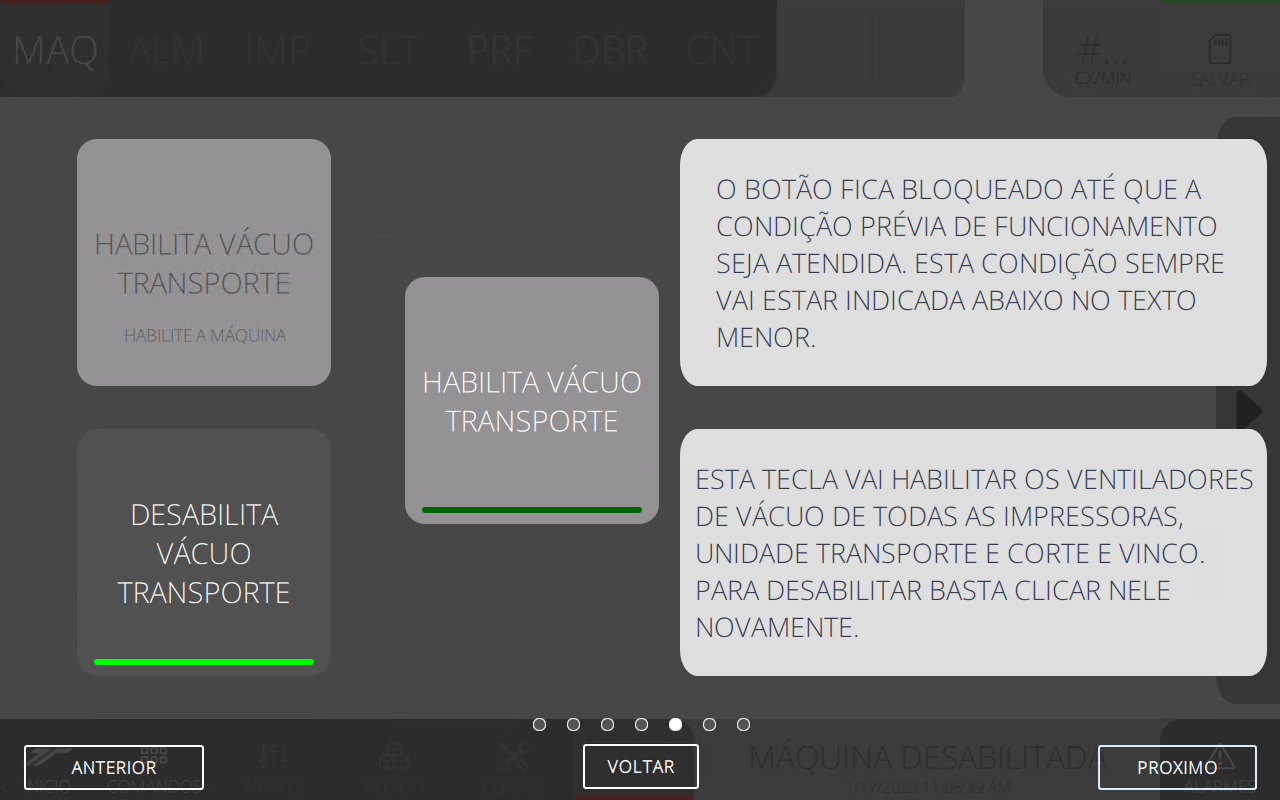
\includegraphics[width=576px,height=360px]{src/imagesFlexo/02-machine/e-5.png}
\end{figure}

\vspace*{\fill}

\newpage
\thispagestyle{fancy}

\vspace*{\fill}

\subsubsection{\small{Habilita skip feed}}

\begin{figure}[h]
  \centering
  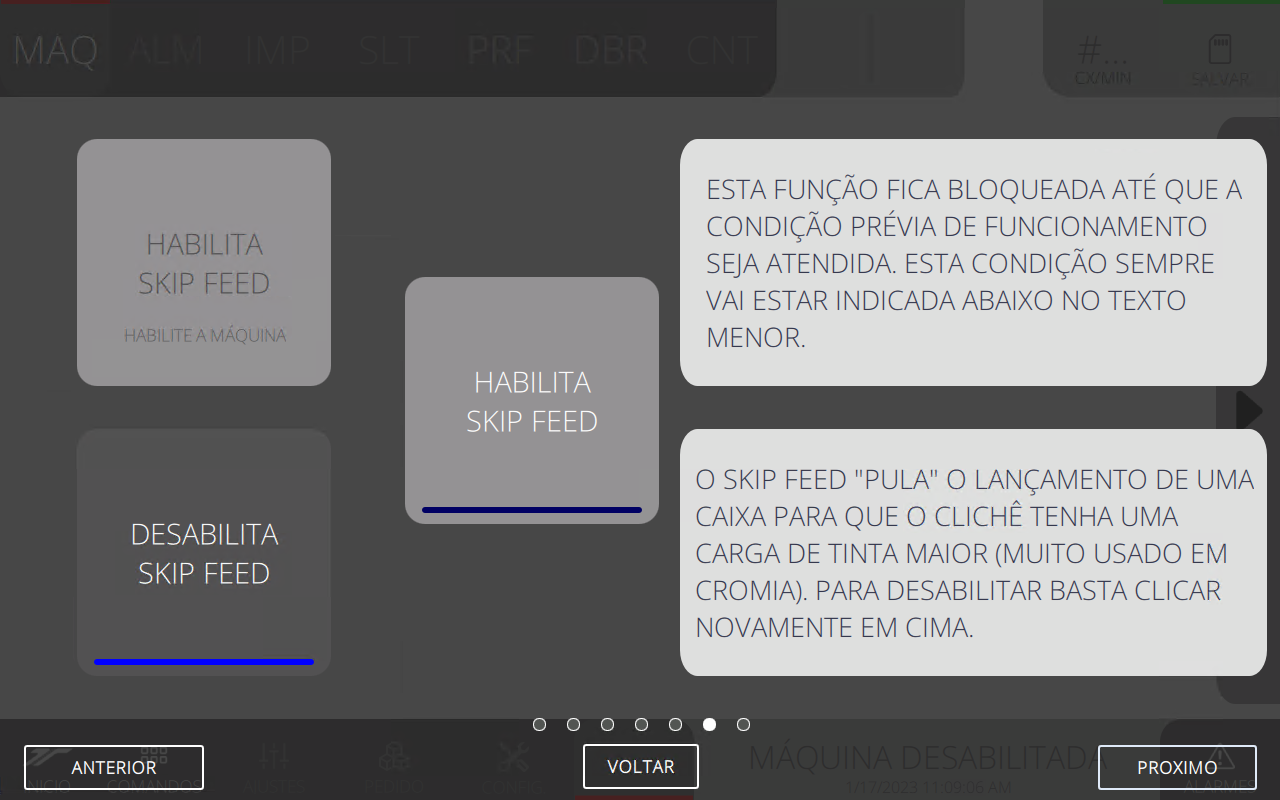
\includegraphics[width=576px,height=360px]{src/imagesFlexo/02-machine/e-6.png}
\end{figure}

\vspace*{\fill}

\newpage
\thispagestyle{fancy}

\vspace*{\fill}

\subsubsection{\small{Liga controle de embuchamento}}

\begin{figure}[h]
  \centering
  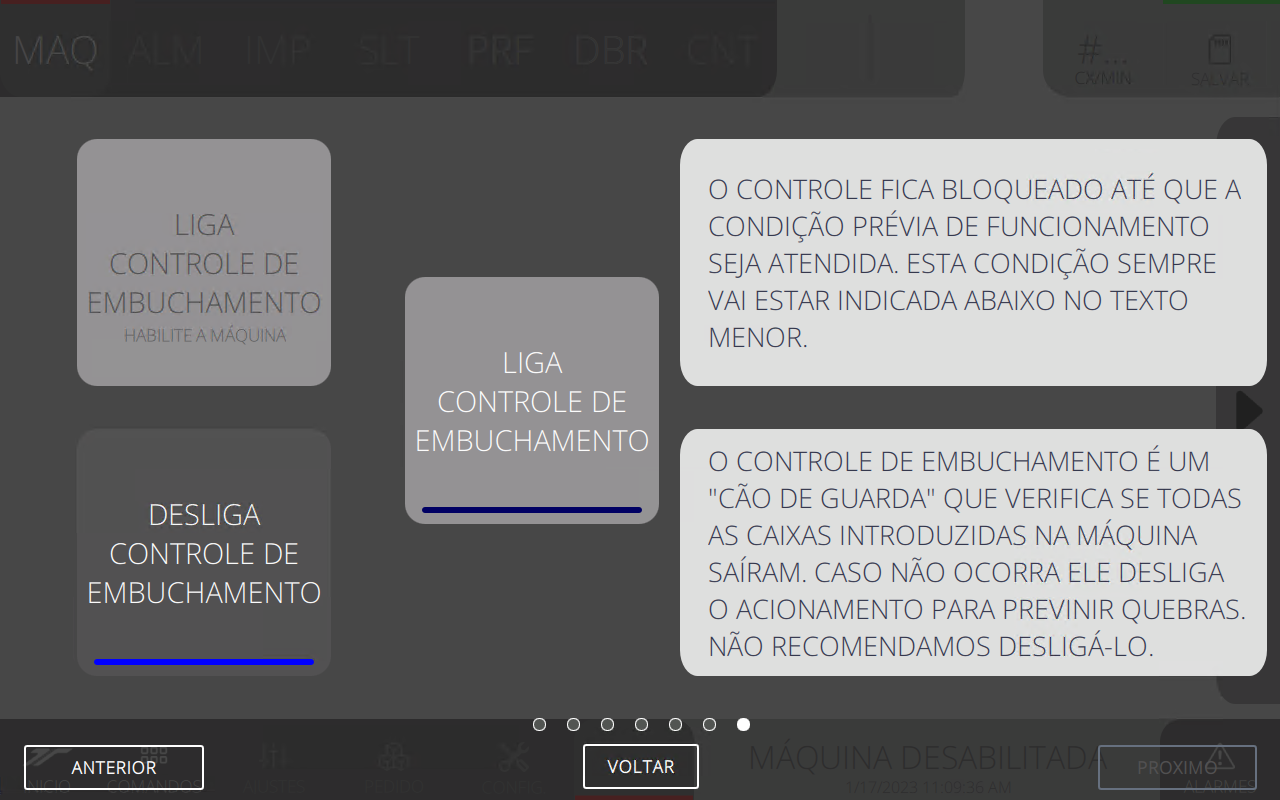
\includegraphics[width=576px,height=360px]{src/imagesFlexo/02-machine/e-7.png}
\end{figure}

\vspace*{\fill}

\newpage
\thispagestyle{fancy}

\vspace*{\fill}

\subsection{Segunda tela comandos de máquina}

Esta tela é acessada pelo botão direito "\textgreater" na tela de comando de máquina. A lógica dos outros menus continua sendo a mesma da sua tela "pai" e para voltar a tela anterior basta clicar no botão esquerdo "\textless{}".

\vspace{10pt}

\begin{figure}[h]
  \centering
  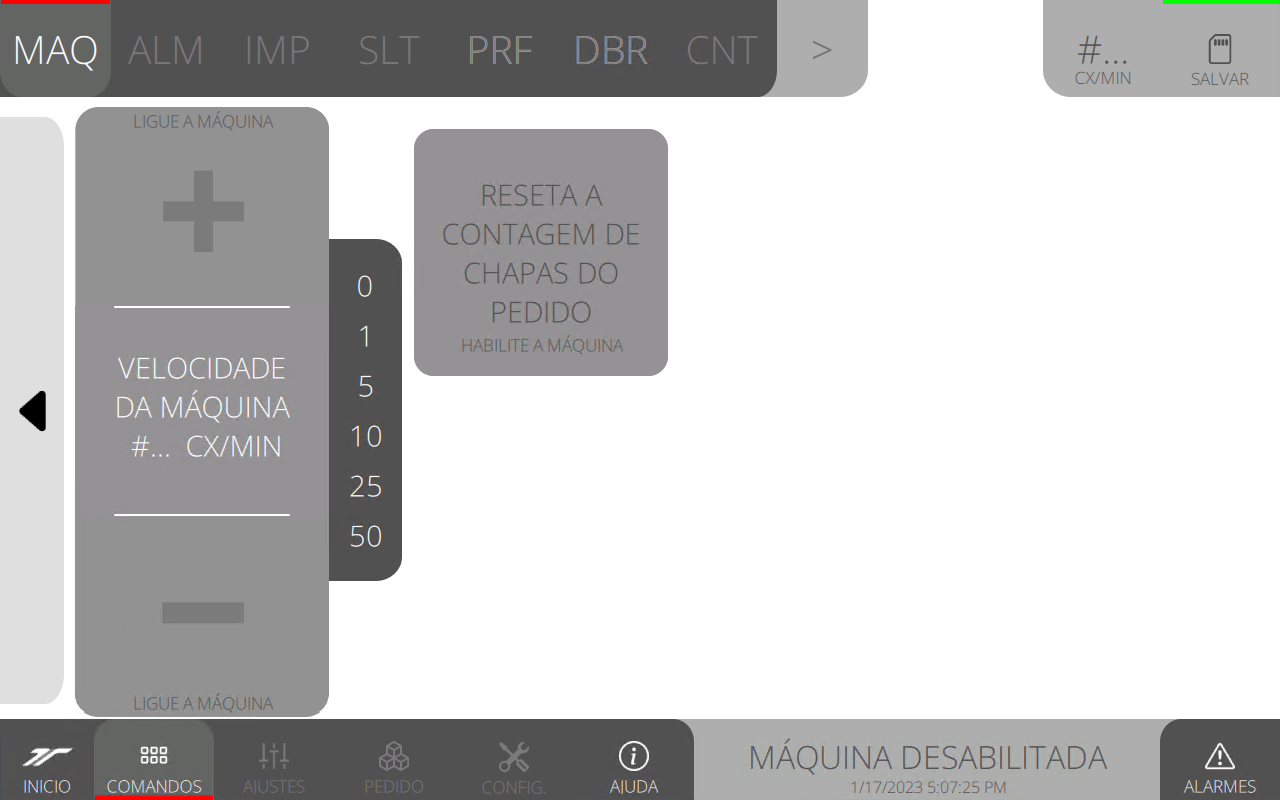
\includegraphics[width=576px,height=360px]{src/imagesFlexo/02-machine/e-Tela-Principal-2.png}
\end{figure}

\newpage
\thispagestyle{fancy}

\vspace*{\fill}

\subsubsection{\small{Reseta a contagem de chapas de pedidos}}

\begin{figure}[h]
  \centering
  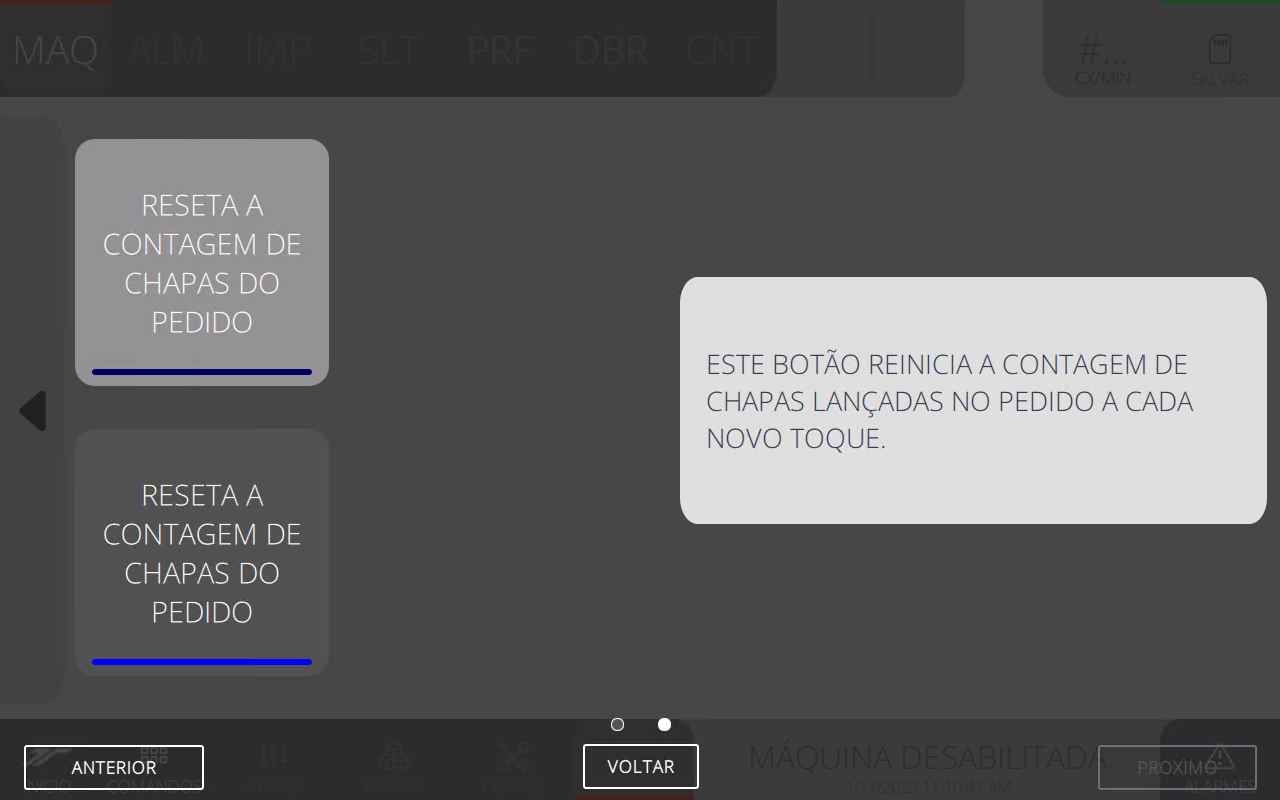
\includegraphics[width=576px,height=360px]{src/imagesFlexo/02-machine/e-9.png}
\end{figure}

\vspace*{\fill}

